% Clase del documento
\documentclass[12pt,twoside,titlepage]{report}


%%%%%%%%%%%%%%%%%%%%%%% Paquetes %%%%%%%%%%%%%%%%%%%%%%%

\usepackage[a4paper,bindingoffset=3mm,bottom=35mm]{geometry}


% Usad \usepackage[dvips]{graphicx} o \usepackage[pdftex]{graphicx} (no ambos)
%\usepackage[dvips]{graphicx} %%% para LaTeX. Las figuras deben estar en formato eps

\usepackage[colorlinks=true,pdftex]{hyperref}   %%% Opcional. Para incluir marcadores y enlaces en el pdf
\usepackage[pdftex]{graphicx}  %%% para pdflatex. Las figuras pueden estar en pdf, jpg, svg y otros formatos


\usepackage[spanish]{babel}

%\usepackage[latin1]{inputenc} % Usad en WinEdt/MikTex
\usepackage[utf8]{inputenc} % Usad en overleaf

%\usepackage[T1]{fontenc}


% Algunos paquetes útiles

\usepackage{amsmath,amssymb}
\usepackage{hyperref}
\usepackage{color}
\usepackage{afterpage}
\usepackage{paralist}
\usepackage{array}
\usepackage{enumerate}
\usepackage{paralist}
\usepackage{enumitem}
\usepackage{float}
\usepackage{setspace}
\usepackage{listings}
\usepackage{algorithm}
\usepackage{algorithmic}
\usepackage{fancyhdr}
\usepackage{rotating}
\usepackage{multirow}


% Otros paquetes

\usepackage{quotchap}
\usepackage{lipsum}

%%%%%%%%%%%%%%%%%%%%%%%%%%%%%%%%%%%%%%%%%%%%%%%%%%%%%%%%






%%%%%%%%%%%%%%%%%%%%%%% Definiciones básicas %%%%%%%%%%%%%%%%%%%%%%%

\newcommand{\nombreautor}{Sergio Simón Fernández}
\newcommand{\nombretutor}{Christian Alcaide Moreno}
\newcommand{\titulotrabajo}{Supercomparator}
\newcommand{\escuela}{IES Gabriel García Márquez}
\newcommand{\escuelalargo}{Escuela Técnica Superior de Ingeniería Informática}
\newcommand{\universidad}{XXX}
\newcommand{\fecha}{Fecha}
\newcommand{\grado}{Ciclo Formativo de Grado Superior en\\Desarrollo de Aplicaciones Multiplataforma}
\newcommand{\curso}{Curso 2022-2024}
\newcommand{\logoUniversidad}{logoURJC.pdf} % logoURJC.eps
\newcommand{\mercadonaPostman}{images/mercadona_postman.png} % logoURJC
\newcommand{\mercadonaRequest}{images/mercadona_request.png} % logoURJC

%%%%%%%%%%%%%%%%%%%%%%%%%%%%%%%%%%%%%%%%%%%%%%%%%%%%%%%%%%%%%%%%%%%%






%%%%%%%%%%%%%%%%%%%%%%%%% Otras definiciones %%%%%%%%%%%%%%%%%%%%%%%%%%

% Definiciones de colores (para hidelinks)
\definecolor{BlueLink}{rgb}{0.165,0.322,0.745}
\definecolor{PinkLink}{rgb}{0.8,0.22,0.5}
\definecolor{gray}{rgb}{0.6,0.6,0.6}


% Enlaces
% \hypersetup{
%     colorlinks=true,
%     linkcolor=blue,
%     urlcolor=blue,
%     linkbordercolor=blue,
%     pdfborderstyle={/S/U/W 1}
% }

\newcommand\blankpage{%
    \newpage
    \null
    \thispagestyle{empty}%
    %\addtocounter{page}{-1}%
    \newpage}


% Texto referencias
\addto{\captionsspanish}{\renewcommand{\bibname}{Bibliografía}}

% Texto Índice de tablas
\addto\captionsspanish{
\def\tablename{Tabla}
\def\listtablename{\'{I}ndice de tablas}
}


\floatname{algorithm}{Algoritmo}

\newfloat{algorithm}{t}{lop}


%\newenvironment{pseudocodigo}[1][htb]
%  {\renewcommand{\algorithmcfname}{Pseudocódig}% Update algorithm name
%   \begin{algorithm}[#1]%
%  }{\end{algorithm}}
  
%%%%%%%%%%%%%%%%%%%%%%%%%%%%%%%%%%%%%%%%%%%%%%%%%%%%%%%%%%%%%%%%%%%%


%%%%%%%%%%%%%%%%%%%%%%% Estilo de código (en Koltin) %%%%%%%%%%%%%%%%%%%%%%%

\usepackage[dvipsnames]{xcolor}
\usepackage{listings}

\lstdefinelanguage{Kotlin}{
  comment=[l]{//},
  commentstyle={\color{gray}\ttfamily},
  emph={filter, first, firstOrNull, forEach, lazy, map, mapNotNull, println},
  emphstyle={\color{OrangeRed}},
  identifierstyle=\color{black},
  keywords={!in, !is, abstract, actual, annotation, as, as?, break, by, catch, class, companion, const, constructor, continue, crossinline, data, delegate, do, dynamic, else, enum, expect, external, false, field, file, final, finally, for, fun, get, if, import, in, infix, init, inline, inner, interface, internal, is, lateinit, noinline, null, object, open, operator, out, override, package, param, private, property, protected, public, receiveris, reified, return, return@, sealed, set, setparam, super, suspend, tailrec, this, throw, true, try, typealias, typeof, val, var, vararg, when, where, while},
  keywordstyle={\color{NavyBlue}\bfseries},
  morecomment=[s]{/*}{*/},
  morestring=[b]",
  morestring=[s]{"""*}{*"""},
  ndkeywords={@Deprecated, @JvmField, @JvmName, @JvmOverloads, @JvmStatic, @JvmSynthetic, Array, Byte, Double, Float, Int, Integer, Iterable, Long, Runnable, Short, String, Any, Unit, Nothing},
  ndkeywordstyle={\color{BurntOrange}\bfseries},
  sensitive=true,
  stringstyle={\color{ForestGreen}\ttfamily},
}

%%%%%%%%%%%%%%%%%%%%%%%%%%%%%%%%%%%%%%%%%%%%%%%%%%%%%%%%%%%%%%%%%%%%





%%%%%%%%%%%%%%%%%%%%%%% Estilo de código (en Python) %%%%%%%%%%%%%%%%%%%%%%%

\definecolor{bg}{rgb}{0.95,0.95,0.95}
\definecolor{mydeepteal}{rgb}{0.16,0.22,0.23}
\definecolor{myteal}{rgb}{0.31,0.44,0.46}
\definecolor{mymediumteal}{rgb}{0.41,0.58,0.60}

\DeclareFixedFont{\ttb}{T1}{txtt}{bx}{n}{12} % for bold
\DeclareFixedFont{\ttm}{T1}{txtt}{m}{n}{12}  % for normal


%\newcommand*{\FormatDigit}[1]{\textcolor{mydeepteal}{#1}}
\newcommand*{\FormatDigit}[1]{\textcolor{black}{#1}}

% Python style for highlighting
\newcommand\mypythonstyle{\lstset{
language=Python,
basicstyle=\ttfamily\small,
%basicstyle=\linespread{1.0}\footnotesize\ttm,
otherkeywords={self},             % Add keywords here
keywordstyle=\bfseries\ttfamily\color{myteal},
%keywordstyle=\ttb\color{myteal},
commentstyle=\itshape\color{myteal},
stringstyle=\color{mydeepteal},
emph={MyClass,__init__},          % Custom highlighting
emphstyle=\ttb\color{mydeepteal},    % Custom highlighting style
% Any extra options here
showstringspaces=false,            %
backgroundcolor=\color{bg},
rulecolor = \color{bg},
%identifierstyle=\color{deepgreen},
breaklines=true,
numbers=left,
numbersep=5pt,
numberstyle=\tiny,
tabsize=4,
xleftmargin=1em,
frame = single,
framesep = 3pt,
framextopmargin=0pt,
framexbottommargin=0pt,
framexleftmargin=0pt,
framexrightmargin=0pt,
fontadjust=true,
basewidth=0.55em, % compactness of code
upquote=true,
}}

% Python environment
\lstnewenvironment{mypython}[1][]
{
\mypythonstyle
\lstset{#1}
}
{}

\newcommand\mypythonstylenormalinline{\lstset{
language=Python,
basicstyle=\ttfamily\normalsize,
%basicstyle=\linespread{1.0}\footnotesize\ttm,
otherkeywords={self},            % Add keywords here
keywordstyle=\bfseries\ttfamily\color{myteal},
%keywordstyle=\ttb\color{myteal},
commentstyle=\itshape\color{mymediumteal},
stringstyle=\color{mydeepteal},
emph={MyClass,__init__},          % Custom highlighting
emphstyle=\ttb\color{mydeepteal},    % Custom highlighting style
% Any extra options here
showstringspaces=false,            %
backgroundcolor=\color{bg},
rulecolor = \color{bg},
%identifierstyle=\color{deepgreen},
breaklines=false,
numbers=left,
numbersep=5pt,
numberstyle=\tiny,
tabsize=4,
xleftmargin=0em,
frame = single,
framesep = 3pt,
framextopmargin=0pt,
framexbottommargin=0pt,
framexleftmargin=0pt,
framexrightmargin=0pt,
fontadjust=true,
%basewidth=0.55em, % compactness of code
upquote=true,
}}

\newcommand\mypythoninline[1]{{\mypythonstylenormalinline\lstinline!#1!}}

%%%%%%%%%%%%%%%%%%%%%%%%%%%%%%%%%%%%%%%%%%%%%%%%%%%%%%%%%%%%%%%%%%%%%%%%%%%%%%




%%%%%%%%%%%%%%%%%%%%%%%%%%%% Comandos definidos por el autor 

\newcommand{\transpuesta}{\mbox{\tiny $\mathsf{T}$}}








%%%%%%%%%%%%%%%%%%%%%%%%%%%%%%%%%%%%%%%%%%%%%%%%%%%%%%%%%%%%%%%%%%%%%%%
%                           Inicio del documento                       
%%%%%%%%%%%%%%%%%%%%%%%%%%%%%%%%%%%%%%%%%%%%%%%%%%%%%%%%%%%%%%%%%%%%%%%


\begin{document}

\pagestyle{plain}




%%%%%%%%%%%%%%%%%%%%%%%%%%%%%%%%%%%% Portada %%%%%%%%%%%%%%%%%%%%%%%%%%%%%%%%%%

%\pagenumbering{gobble}
%\pagenumbering{arabic}

% Universidad, Facultad
\begin{titlepage}
	\selectlanguage{spanish}


	% logo
	\begin{center}
		
\includegraphics[scale=1]{figuras/logo_ggm}
	\end{center}

	%\bigskip

	\begin{center}
		\begin{LARGE}
			\escuela \\
		\end{LARGE}
	\end{center}

	\bigskip
	\bigskip

	% Grado
	\begin{center}
		\begin{large}
			\textbf{\grado}\\
		\end{large}
	\end{center}

	% Curso
	\begin{center}
		\begin{large}
			\textbf{\curso}\\
		\end{large}
	\end{center}

	\bigskip

	\textbf{\begin{center}
			\begin{large}
				\textbf{Trabajo Fin de Ciclo}
			\end{large}
		\end{center}}

	\bigskip
	\bigskip
	\bigskip

	% Nombre del TFG
	\begin{center}
		\textbf{\begin{large}
				\MakeUppercase{\titulotrabajo}\\
			\end{large}}
	\end{center}

	% Nombre del autor
	\vspace{\fill}
	\begin{center}
		\textbf{Autor: \nombreautor}\\ \smallskip
		% Tutor
		\textbf{Tutor: \nombretutor}\\
		% Añadir segundo tutor si hubiera


		\bigskip

		% Fecha
		%\textbf{\fecha}\\
	\end{center}
\end{titlepage}


%%%%%%%%%%%%%%%%%%%%%%%% Opcional %%%%%%%%%%%%%%%%%%%%%%
%\blankpage

%\thispagestyle{empty}
%\begin{center}

% Nombre del trabajo
%\textbf{\begin{large}
%\MakeUppercase{\titulotrabajo}\\*
%\end{large}}
%\vspace*{0.2cm}
%\vspace{5cm}

% Nombre del autor y del tutor
%\large Autor: \nombreautor \\* \medskip
%\large Tutor: \nombretutor \\*

%\vfill

% Escuela, universidad y fecha
%\escuelalargo \\ \smallskip
%\universidad \\
%\vspace{1cm}
%\fecha \\

%\clearpage

%\end{center}
%%%%%%%%%%%%%%%%%%%%%%%%%%%%%%%%%%%%%%%%%%%%%%%%%%%%%%%%

\hypersetup{pageanchor=true}

\normalsize
\afterpage{\blankpage} % Se deben añadir página en blanco para que lo capítulos de la memoria o estas secciones introductorias empiecen en páginas impares

%%%%%%%%%%%%%%%%%%%%%%%%%%%%%%%%%%%%%%%%%%%%%%%%%%%%%%%%%%%%%%%%%%%%%%%%%%%%%%%





% Estilo de párrafo de los capítulos
\setlength{\parskip}{0.75em}
\renewcommand{\baselinestretch}{1.25}
% Interlineado simple
\spacing{1}

\pagenumbering{Roman}
\setcounter{page}{2}


%%%%%%%%%%%%%%%%%%%%%%%%% Agradecimientos o dedicatoria %%%%%%%%%%%%%%%%%%%%%%%%%%%

\chapter*{Agradecimientos}

Breves agradecimientos o dedicatoria.

\afterpage{\blankpage}

%%%%%%%%%%%%%%%%%%%%%%%%%%%%%%%%%%%%%%%%%%%%%%%%%%%%%%%%%%%%%%%%%%%%%%%%%%%%%%%%%%%






%%%%%%%%%%%%%%%%%%%%%%%%%%%%%%%%%%%% Resumen %%%%%%%%%%%%%%%%%%%%%%%%%%%%%%%%%%%%%%

\chapter*{Resumen}

Breve resumen del Trabajo de Fin de Grado (TFG). Recomendable entre 250-300 palabras, conteniendo los principales objetivos y resultados derivados del mismo.

Para este proyecto se ha buscado poder realizar comparaciones entre productos de distintas páginas de supermercados. Para ello, se han realizado consultas para obtener la información necesaria

\mbox{} \bigskip

\noindent \textbf{Palabras clave}:
\begin{compactitem}
	\item Python
	\item Ciberseguridad
	\item Aprendizaje automático (pueden ser varias)
	\item $\ldots$
\end{compactitem}

\afterpage{\blankpage}

%%%%%%%%%%%%%%%%%%%%%%%%%%%%%%%%%%%%%%%%%%%%%%%%%%%%%%%%%%%%%%%%%%%%%%%%%%%%%%%%%%%





%%%%%%%%%%%%%%%%%%%%%%%%%%%%%%%%%%%% Índices %%%%%%%%%%%%%%%%%%%%%%%%%%%%%%%%%%%%

% Estilo de párrafo de los Índices
\setlength{\parskip}{1pt}
\renewcommand{\baselinestretch}{1}
\renewcommand{\contentsname}{Índice de contenidos}


% Índice de contenidos
\tableofcontents
\afterpage{\blankpage}

% Índice de tablas (OPCIONAL)
\listoftables
\afterpage{\blankpage}
\addcontentsline{toc}{chapter}{\noindent \listtablename}

% Índice de figuras (OPCIONAL)
\listoffigures
\afterpage{\blankpage}
\addcontentsline{toc}{chapter}{\listfigurename}

% Índice de códigos/algoritmos (OPCIONAL).   El término "Códigos" se puede cambiar por "Métodos", "Funciones", "Algoritmos", etc.
\renewcommand\lstlistlistingname{Códigos}
\renewcommand\lstlistingname{Código}
\renewcommand\lstlistlistingname{Índice de códigos}

\lstlistoflistings
\afterpage{\blankpage}
\addcontentsline{toc}{chapter}{\lstlistlistingname}


% En este documento (de momento) no se ha considerado incluir un índice de algoritmos/pseudocódigos, como el que aparece en \ref{AdditionalLouvain}

%%%%%%%%%%%%%%%%%%%%%%%%%%%%%%%%%%%%%%%%%%%%%%%%%%%%%%%%%%%%%%%%%%%%%%%%%%%%%%%%%%%





%%%%%%%%%%%%%%%%%%%%%%% Cabeceras y pies de página (Opcional) %%%%%%%%%%%%%%%%%%%%%%%

%\setlength{\headheight}{15.2pt}
\pagestyle{fancy}


\renewcommand{\chaptermark}[1]{\markboth{Capítulo \thechapter.\ #1}{}}

\pagestyle{fancy}
\fancyhf{}
\fancyhead[LO]{\leftmark}
\fancyhead[RO]{}
\fancyhead[RE]{\nouppercase\rightmark}
\fancyhead[LE]{}
\fancyfoot[C]{\thepage}

%%%%%%%%%%%%%%%%%%%%%%%%%%%%%%%%%%%%%%%%%%%%%%%%%%%%%%%%%%%%%%%%%%%%%%%%%%%%%%%%%%%%






%%%%%%%%%%%%%%%%%%%%%%%%%%%%%% Capítulos de la memoria %%%%%%%%%%%%%%%%%%%%%%%%%%%%%



% Capítulo 1
\chapter{Introducción}


%%%%%%%%%%%%%%%%%%%%%%%%%%%%%%%%%%%%%%%%%%%%%%%%%%%%%%%%%%%%%%%%%%%%%%%%%%

% Estilo resto de páginas
\pagestyle{fancy}


% Estilo de párrafo de los capítulos
\setlength{\parskip}{0.75em}
\renewcommand{\baselinestretch}{1.25}
% Interlineado simple
\spacing{1}
% Numeración contenido
\pagenumbering{arabic}
\setcounter{page}{1}

%%%%%%%%%%%%%%%%%%%%%%%%%%%%%%%%%%%%%%%%%%%%%%%%%%%%%%%%%%%%%%%%%%%%%%%%%%



Se puede añadir texto antes de empezar la primera sección.


\section{Contexto y alcance}

Contexto. Situar al lector. Objetivo general y alcance del trabajo.

Hay que ir poco a poco acotando el contexto donde se desarrolla el proyecto. No se debe sobreentender que el evaluador de la memoria sabe del tema. Escribid el texto para la abuela.


\section{Estructura del documento}

La estructura del TFG no es fija. El tutor indicará una estructura adecuada dependiendo del trabajo concreto.

Se puede incluir dentro de cada apartado secciones adicionales. La copia en papel de la memoria del TFG será encuadernada en pasta dura de color azul (p.e. encuadernación tipo chanel). La portada, que puede ser una pegatina transparente, seguirá el modelo que se adjunta, que incluye el escudo y nombre de la URJC, la titulación cursada por el alumno, el curso académico, el título del TFG, el autor y el o los directores/tutores.



% \afterpage{\blankpage} % puede generar problema en índice de contenidos
% \newpage







% Capítulo 2
\chapter{Objetivos}


% Objetivos generales y específicos del trabajo.


\section{Objetivo general}

\begin{itemize}

	\item[1] Obtener productos de distintos supermercados
	\item[2] Permitir registro e inicio de sesión online
	\item[3] Permitir de manera automatizada varias consultas de distintos productos
	\item[4] Almacenar una copia de su configuración como sus listas de productos guardadas
	\item[5] Permitir a los usuarios subir información adicional sobre los productos para mejorar las búsquedas y su información

\end{itemize}


\section{Objetivos específicos}

\begin{itemize}

	\item[3.1] Permitir crear listas de consultas preconfiguradas para realizar búsquedas simultáneas de varios productos
	\item[4.1] Almacenar la configuración del usuario en Firebase para hacerla siempre disponible
	\item[5.1] Ver un historial de precios de cada producto
	\item[5.1] Ver valor nutricional de cada producto obteniendo la información de medios externos

\end{itemize}

\blankpage


% Capítulo 3
\chapter{Estado del arte}

\section{Super más barato}

Mi principal fuente de inspiración para el desarrollo del proyecto ha sido, en gran medida, la página web de Super más barato\cite{Super más barato}. En este sitio, tenemos la capacidad de elegir los supermercados que deseamos para comparar los precios de los productos. Al buscarlos, encontraremos el nombre del producto, una imagen del mismo, su precio y el precio por cantidad.

\section{Soysuper}

Soysuper\cite{Soysuper} es una web que cuenta con aplicaciones disponibles tanto para Android como iOS. Aunque ofrece las funciones básicas de búsqueda y comparación entre supermercados, destaca por una característica innovadora: la posibilidad de agregar productos a la cesta del supermercado directamente desde su página web. Actualmente, esta función solo está disponible para productos de la misma cadena de supermercados. Otra característica notable es la presencia de una variedad de productos recomendados, sin necesidad de realizar búsquedas previas, lo que sugiere la existencia de una base de datos propia que abarca todos los productos de los supermercados, o al menos, de búsquedas anteriores.


% Capítulo 4
\chapter{Metodología}
\label{chap:contenidos}




\section{Relación con el Ciclo}

% Citar una referencia
Hola, esto es una referencia bibliográfica \cite{libro_calculo}. Se recomienda leer ``The Not So Short Introduction to \LaTeX'' \cite{Oetiker2007} (existen versiones más modernas).


% Insertar una figura
\begin{figure}
	\centering
	\includegraphics[width=0.75\textwidth,clip=true]{\logoUniversidad}
	\caption{Logo de la Universidad.}
	\label{fig:logo_universidad}
\end{figure}

% Referenciar una etiqueta (label)
Las tablas y figuras deben presentarse en el texto, referenciadas y numeradas. La descripción de una figura debe ir posicionada debajo de la misma. Las descripciones de tablas pueden aparecer encima o debajo de las mismas (pero de forma consistente en todo el documento).

En las tablas se recomienda evitar líneas verticales y usar pocas horizontales.

La figura~\ref{fig:logo_universidad} se utiliza en la portada. \LaTeX ubica automáticamente las tablas y figuras. Para ello emplea reglas basadas en la experiencia de profesionales de la edición de textos. Podemos forzar su ubicación, pero en general es recomendable usar la ubicación sugerida por el sistema \LaTeX. Usad gráficos vectoriales siempre que podáis.





\begin{figure}
	\centering

	\begin{minipage}{0.45\textwidth}
		\centering

		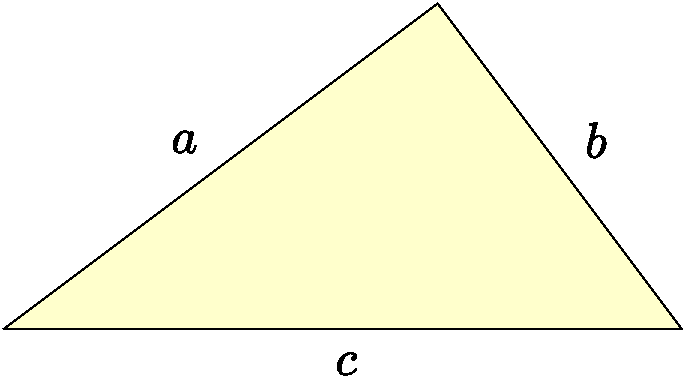
\includegraphics[clip=true,width=\textwidth]{triangulo_grande_bb.pdf}\\

		\footnotesize (a)
	\end{minipage}
	\hfill
	\begin{minipage}{0.45\textwidth}
		\centering
		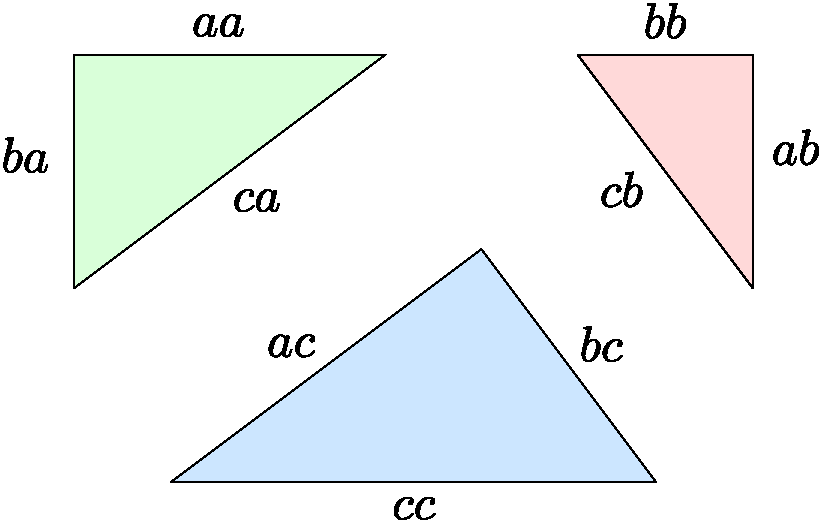
\includegraphics[clip=true,width=\textwidth]{triangulos_separados_bb.pdf}\\

		\footnotesize (b)
	\end{minipage}

	\bigskip

	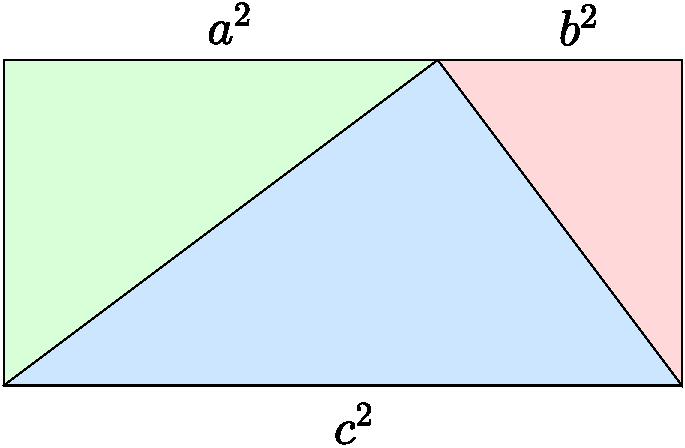
\includegraphics[clip=true,width=0.5\textwidth]{triangulos_unidos_bb.pdf}\\
	\footnotesize (c)

	\caption{Ejemplo con varias figuras. Demostración visual del teorema de Pitágoras. En (a) tenemos un triángulo rectángulo con hipotenusa $c$ y catetos $a$ y $b$. En (b) se muestra tres copias escaladas del mismo triángulo. El verde se ha escalado por $a$, el rojo/rosa por $b$, y el azul por $c$. En (c) se juntan los triángulos de (b) para formar un rectángulo cuya base es $c^{2}$, pero también $a^{2} + b^{2}$. Por tanto, $a^{2} + b^{2} = c^{2}$.}\label{fig:teoremapitagoras}
\end{figure}





\section{Introducción a la Tecnología/Aplicación utilizada}

\subsection{Web scraping}
\label{sec:WebScraping}

Para el proyecto \titulotrabajo \space se ha necesitado usar \textbf{web scraping}, pero antes de hablar como se ha usado usaré un pequeño ejemplo que da la página web Geeksforgeeks que es el WebScraping \cite{WebScraping}

\begin{itemize}
	\item Imaginemos que necesitas obtener información de un sitio web. Copiar y pegar puede servir para pequeñas cantidades, pero ¿qué hacer si requieres grandes cantidades de datos de manera rápida? En ese caso, copiar y pegar simplemente no es una opción viable. Ahí es donde entra en juego el Web Scraping. A diferencia del tedioso proceso manual de recopilación de datos, el Web Scraping emplea técnicas automatizadas para extraer miles o incluso millones de conjuntos de datos en un lapso de tiempo mucho más corto.
\end{itemize}

En el proyecto se han utilizado dos métodologias de web scraping:

\begin{itemize}
	\item Llamado de una api del comercio
	\item Filtrado del html del comercio
\end{itemize}

Cuando solicitamos datos al api del comercio, estos nos llegan en formato json, describiendo los productos consultados. A partir de esta información, llevamos a cabo una conversión a un objeto Kotlin. Este objeto almacena la información completa o parcial del producto, dependiendo del alcance de la consulta y la relevancia de los datos obtenidos.

El proceso de filtrado mediante html es bastante similar. Realizamos una consulta que nos devuelve todo el contenido de la página web del comercio. Luego, trabajamos con este html para extraer los datos relevantes que deseamos almacenar en un objeto de Kotlin. Este filtrado se lleva a cabo utilizando las etiquetas html, las cuales están asociadas a clases css que nos permiten distinguir los distintos campos de la página y, por ende, extraer los datos que nos interesan.


\subsection{Selenium WebDriver}
\label{sec:Selenium}

Selenium WebDriver es según la página web \textit{El blog de python} \cite{Selenium WebDriver} es una herramienta de automatización de pruebas que permite interactuar con aplicaciones web de forma automatizada.

La elección de Selenium WebDriver para nuestro proyecto se fundamenta en su funcionamiento interno. Esta herramienta opera mediante la utilización de un controlador de navegador, como Firefox, para ejecutar las pruebas de forma automática. Crea un navegador virtual que nos permite ejecutar el JavaScript necesario en aquellas páginas que requieran este tipo de interacción.

\section{Desarrollo del proyecto}

\newpage
% También con \pagebreak



\subsection{Código}


\begin{mypython}[float={!t},caption={Titulo del algoritmo/código.},label={alg:etiqueta}]
	def sum_list_limits_1(a, lower, upper):
	if lower > upper:
	return 0
	else:
	return a[upper] + sum_list_limits_1(a, lower, upper - 1)
\end{mypython}


\begin{lstlisting}[caption={Simple code listing.}, label={alg:examples1}, language=Kotlin]
	// this is a simple code listing:
	println("hello kotlin from latex")
	\end{lstlisting}

El código~\ref{alg:etiqueta} es un ejemplo en Python.

Código Kotlin de ejemplo \ref{alg:examples1}


\begin{algorithm}
	\begin{algorithmic}[1]
		\STATE $\forall i \in V$, \ let $i$ be an isolated community
		\STATE $o=permutation(V)$
		\FOR{$k \ \in \ o$}
		\STATE search in $A$ all the neighbours of $k$, $j$
		\STATE $\forall j$, calculate $\Delta Q_k(j)$ in matrix $\mathcal{M}$
		\STATE $j^*=\{ \ j \ | \ \Delta Q_k(j^*)=\max_j\{Q_k(j)\} \ \}$
		\IF{$\Delta Q_k(j^*)>0$}
		\STATE{Move node $k$ to $j^*$ 's community}
		\ELSE
		\STATE{$k$ remains in its community}
		\ENDIF
		\ENDFOR
	\end{algorithmic}\caption{\textit{Additional Louvain} \textbf{input}=$\left(A, \ \mathcal{M}\right)$ \textbf{output}=$P$}
	\label{alg:AdditionalLouvain}
\end{algorithm}
En el algoritmo~\ref{alg:AdditionalLouvain} aparece un ejemplo en pseudocódigo.











% Nuevo capítulo
\chapter{Resultados y discusión (opcional)}
\label{sec:resulObtenidos}


En esta sección se describe los resultados obtenidos en el TFG, en caso de realizar propuestas para su resolución. Puede sustituirse por ejemplos u omitirse.

Se deben incluir las pruebas realizadas.

\blankpage

% Nuevo capítulo

\chapter{Conclusiones}

% En este capítulo se detallan las conclusiones derivadas del TFG y la propuesta de posibles trabajos futuros.

% Las citas del texto Autor \cite{giaquinta}, Autor \cite{fortune}, Autor \cite{fortuneB}, Autor \cite{mitchell} y Autor \cite{morrey} deben ir referenciadas en la bibliografia.


\section{Informe post-mortem}

\subsection{Lo que ha ido bien}

\begin{itemize}
	\item Argumento a favor 1.

	\item Argumento a favor 2.

	\item Argumento a favor 3.
\end{itemize}

\subsection{Lo que ha ido mal}

\begin{itemize}

	\item Elección de un framework demasiado reciente.

	      \begin{itemize}

		      \item Para el desarrollo de la aplicación, elegí la opción de usar Kotlin Multiplataforma. Mi principal motivación fue poder aprender a desarrollar aplicaciones multiplataforma, escribiendo el código una vez y ejecutándolo en Android, iOS, Escritorio e incluso Web con una única implementación.

		            % 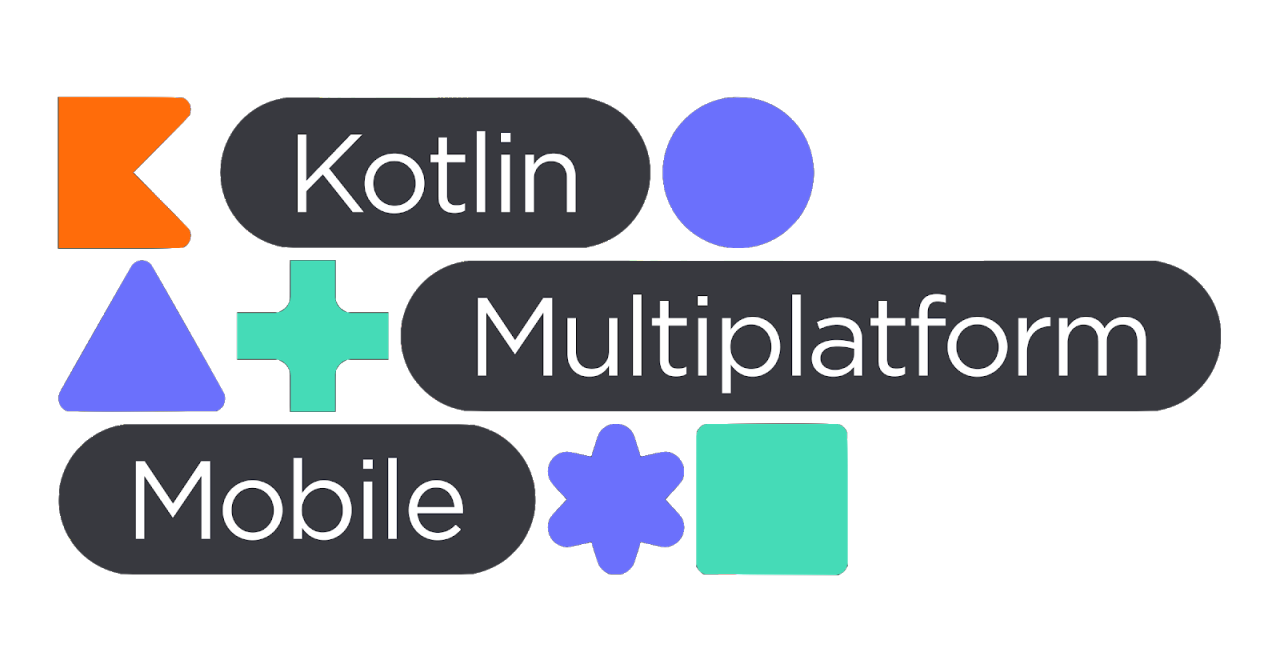
\includegraphics[width=\textwidth]{images/kotlin_multiplataform_logo.png}

		      \item La experiencia resultó ser muy tediosa, ya que encontrar información sobre las librerías y cómo usarlas fue complicado. Pude encontrar una recopilación de librerías compatibles con Kotlin Multiplataforma en el repositorio \textit{Awesome Kotlin Multiplatform} \cite{kmp-awesome}, ya que las librerías de Kotlin regulares no son compatibles.

		      \item La importación también era diferente. Me costó entenderla; por ejemplo, la siguiente línea muestra cómo importar una librería en Gradle (Kotlin) y en Version Catalog (Kotlin-Multiplatform):

		            \begin{lstlisting}[caption={Ejemplo de importación de librerías en Gradle.}, label={alg:gradle.kts-examples}, language=Kotlin]
val voyagerVersion = "1.0.0"

implementation
("cafe.adriel.voyager:voyager-navigator:$voyagerVersion")
\end{lstlisting}

		            \begin{lstlisting}[caption={Ejemplo de importación de librerías en Version Catalog.}, label={alg:libs.versions.kts-examples}, language=Kotlin]
// libs.versions.toml					

voyager = "1.0.0"

voyager = { group = "cafe.adriel.voyager"  
name = "voyager-navigator", version.ref = "coil"}

//build.gradle.kts (Module :app)

implementation(libs.voyager)
\end{lstlisting}

		      \item La escasa documentación sobre cómo usar el framework, sumada a que la implementación de la interfaz gráfica era ligeramente distinta y tenía limitaciones en comparación con Android, me llevó a abandonar la idea de desarrollar la aplicación en Kotlin Multiplataforma.

	      \end{itemize}

	\item Consultas poco estandarizadas e inconvenientes

	      \begin{itemize}

		      \item Para el proyecto \titulotrabajo, se han llevado a cabo múltiples consultas mediante web scraping (véase la sección \ref{sec:WebScraping}). Sin embargo, cada página presenta sus propias particularidades, lo que demanda métodos distintos para extraer la información deseada.

		            Idealmente, habría sido beneficioso que todas las páginas dispusieran de una api que proporcionara un archivo json con los datos de los productos. Esto habría simplificado considerablemente la obtención de la información y mejorado el rendimiento de la aplicación. A pesar de ello, en algunos casos me he visto en la necesidad de filtrar el archivo json debido a su extensión, ya que su transformación completa a una clase de Kotlin no aportaría información relevante.

		            En aquellos casos en los que la api no proporciona un archivo json, se nos suministra el html puro de la página, el cual debemos filtrar según sus clases de css.

		      \item El principal inconveniente ha sido con la página web de Mercadona. En esta página, las consultas no funcionaban debido a que se necesita JavaScript para poder ver el contenido de la página. A continuación, dejo un ejemplo de lo que nos devuelve una consulta haciendo una petición GET:


			  \begin{figure}[htbp]
				\centering
				\includegraphics[width=\linewidth]{\mercadonaPostman}
				\caption{Petición a la API de Mercadona}
				\label{fig:mercadonaPostman}
			\end{figure}

			\begin{figure}[htbp]
				\centering
				\includegraphics[width=\linewidth]{\mercadonaRequest}
				\caption{Respuesta de la petición a la API de Mercadona}
				\label{fig:mercadonaRequest}
			\end{figure}

		      \item Para llevar a cabo las consultas necesarias, he tenido que recurrir a Selenium (consulte la sección \ref{sec:Selenium}). Sin embargo, esto ha representado un gran inconveniente, ya que no puedo ejecutar la biblioteca de manera nativa en Android. La solución que he encontrado es asociar las búsquedas a una API en un servidor.

	      \end{itemize}

\end{itemize}

\subsection{Discusión}

En función de lo anterior, qué cambiaría si empezara hoy el proyecto de nuevo.

\section{Trabajos futuros}

Enumera los puntos abiertos y que no se han resuelto. Indica si darían lugar a otro proyecto y de qué forma se podría acotar.

\lipsum[1-18]
\blankpage



%%%%%%%%%%%%%%%%%%%%%%%%%%%%%%% Bibliografía %%%%%%%%%%%%%%%%%%%%%%%%%%%%%%%
\phantomsection
\addcontentsline{toc}{chapter}{Bibliografía}

\begin{thebibliography}{99} % Ajusta el número según el máximo número de referencias
	\bibitem{kmp-awesome} Terrakok. \textit{Awesome Kotlin Multiplatform}, 2021. \href{https://github.com/terrakok/kmp-awesome}{Fuente}
	\bibitem{WebScraping} Geeksforgeeks. \textit{What is Web Scraping and How to Use It?}, 07 Mar, 2024 \href{https://www.geeksforgeeks.org/what-is-web-scraping-and-how-to-use-it/}{Fuente}
	\bibitem{Selenium WebDriver} El blog python \textit{Guía de Selenium WebDriver en Python para automatizar pruebas web} \href{https://elblogpython.com/tecnologia/guia-de-selenium-webdriver-en-python-para-automatizar-pruebas-web/}{Fuente}
	\bibitem{Super más barato} Super más barato. \textit{Super más barato} \href{https://supermasbarato.es/}{Fuente}
	\bibitem{Soysuper} Soysuper \textit{Soysuper más barato} \href{https://supermasbarato.es/}{Fuente}
\end{thebibliography}



% No expandir elementos para llenar toda la página
\raggedbottom
\afterpage{\blankpage}

\newpage

%%%%%%%%%%%%%%%%%%%%%%%%%%%%%%% Apéndices %%%%%%%%%%%%%%%%%%%%%%%%%%%%%%%

\appendix

\phantomsection
\addcontentsline{toc}{chapter}{Apéndices}

\mbox{}
\vfill
\begin{center}
	\begin{Huge}
		\textbf{Apéndices}
	\end{Huge}
\end{center}
\vfill
\mbox{}
\thispagestyle{empty}

\newpage
\mbox{}
\thispagestyle{empty}
\newpage


% Primer apéndice
\chapter{Este es el primer apéndice}
\label{sec:apendice}


\section{Ejemplo de sección}

Sección del apéndice




% Fin del documento
\end{document}
